\section{Sistema Completo do Filtro Ativo}

O sistema completo � ilustrado na Figura \ref{fig:Tudao_lado_1.png}. Nesta figura pode ser observado todos os passos de c�lculo necess�rios para a determina��o das correntes de refer�ncia de um filtro ativo do tipo \textit{shunt}, juntamente com a opera��o de controle do compensador. 

\begin{figure}[!htbp] %Esquema de um filtro passivo gen�rico
	\centering
	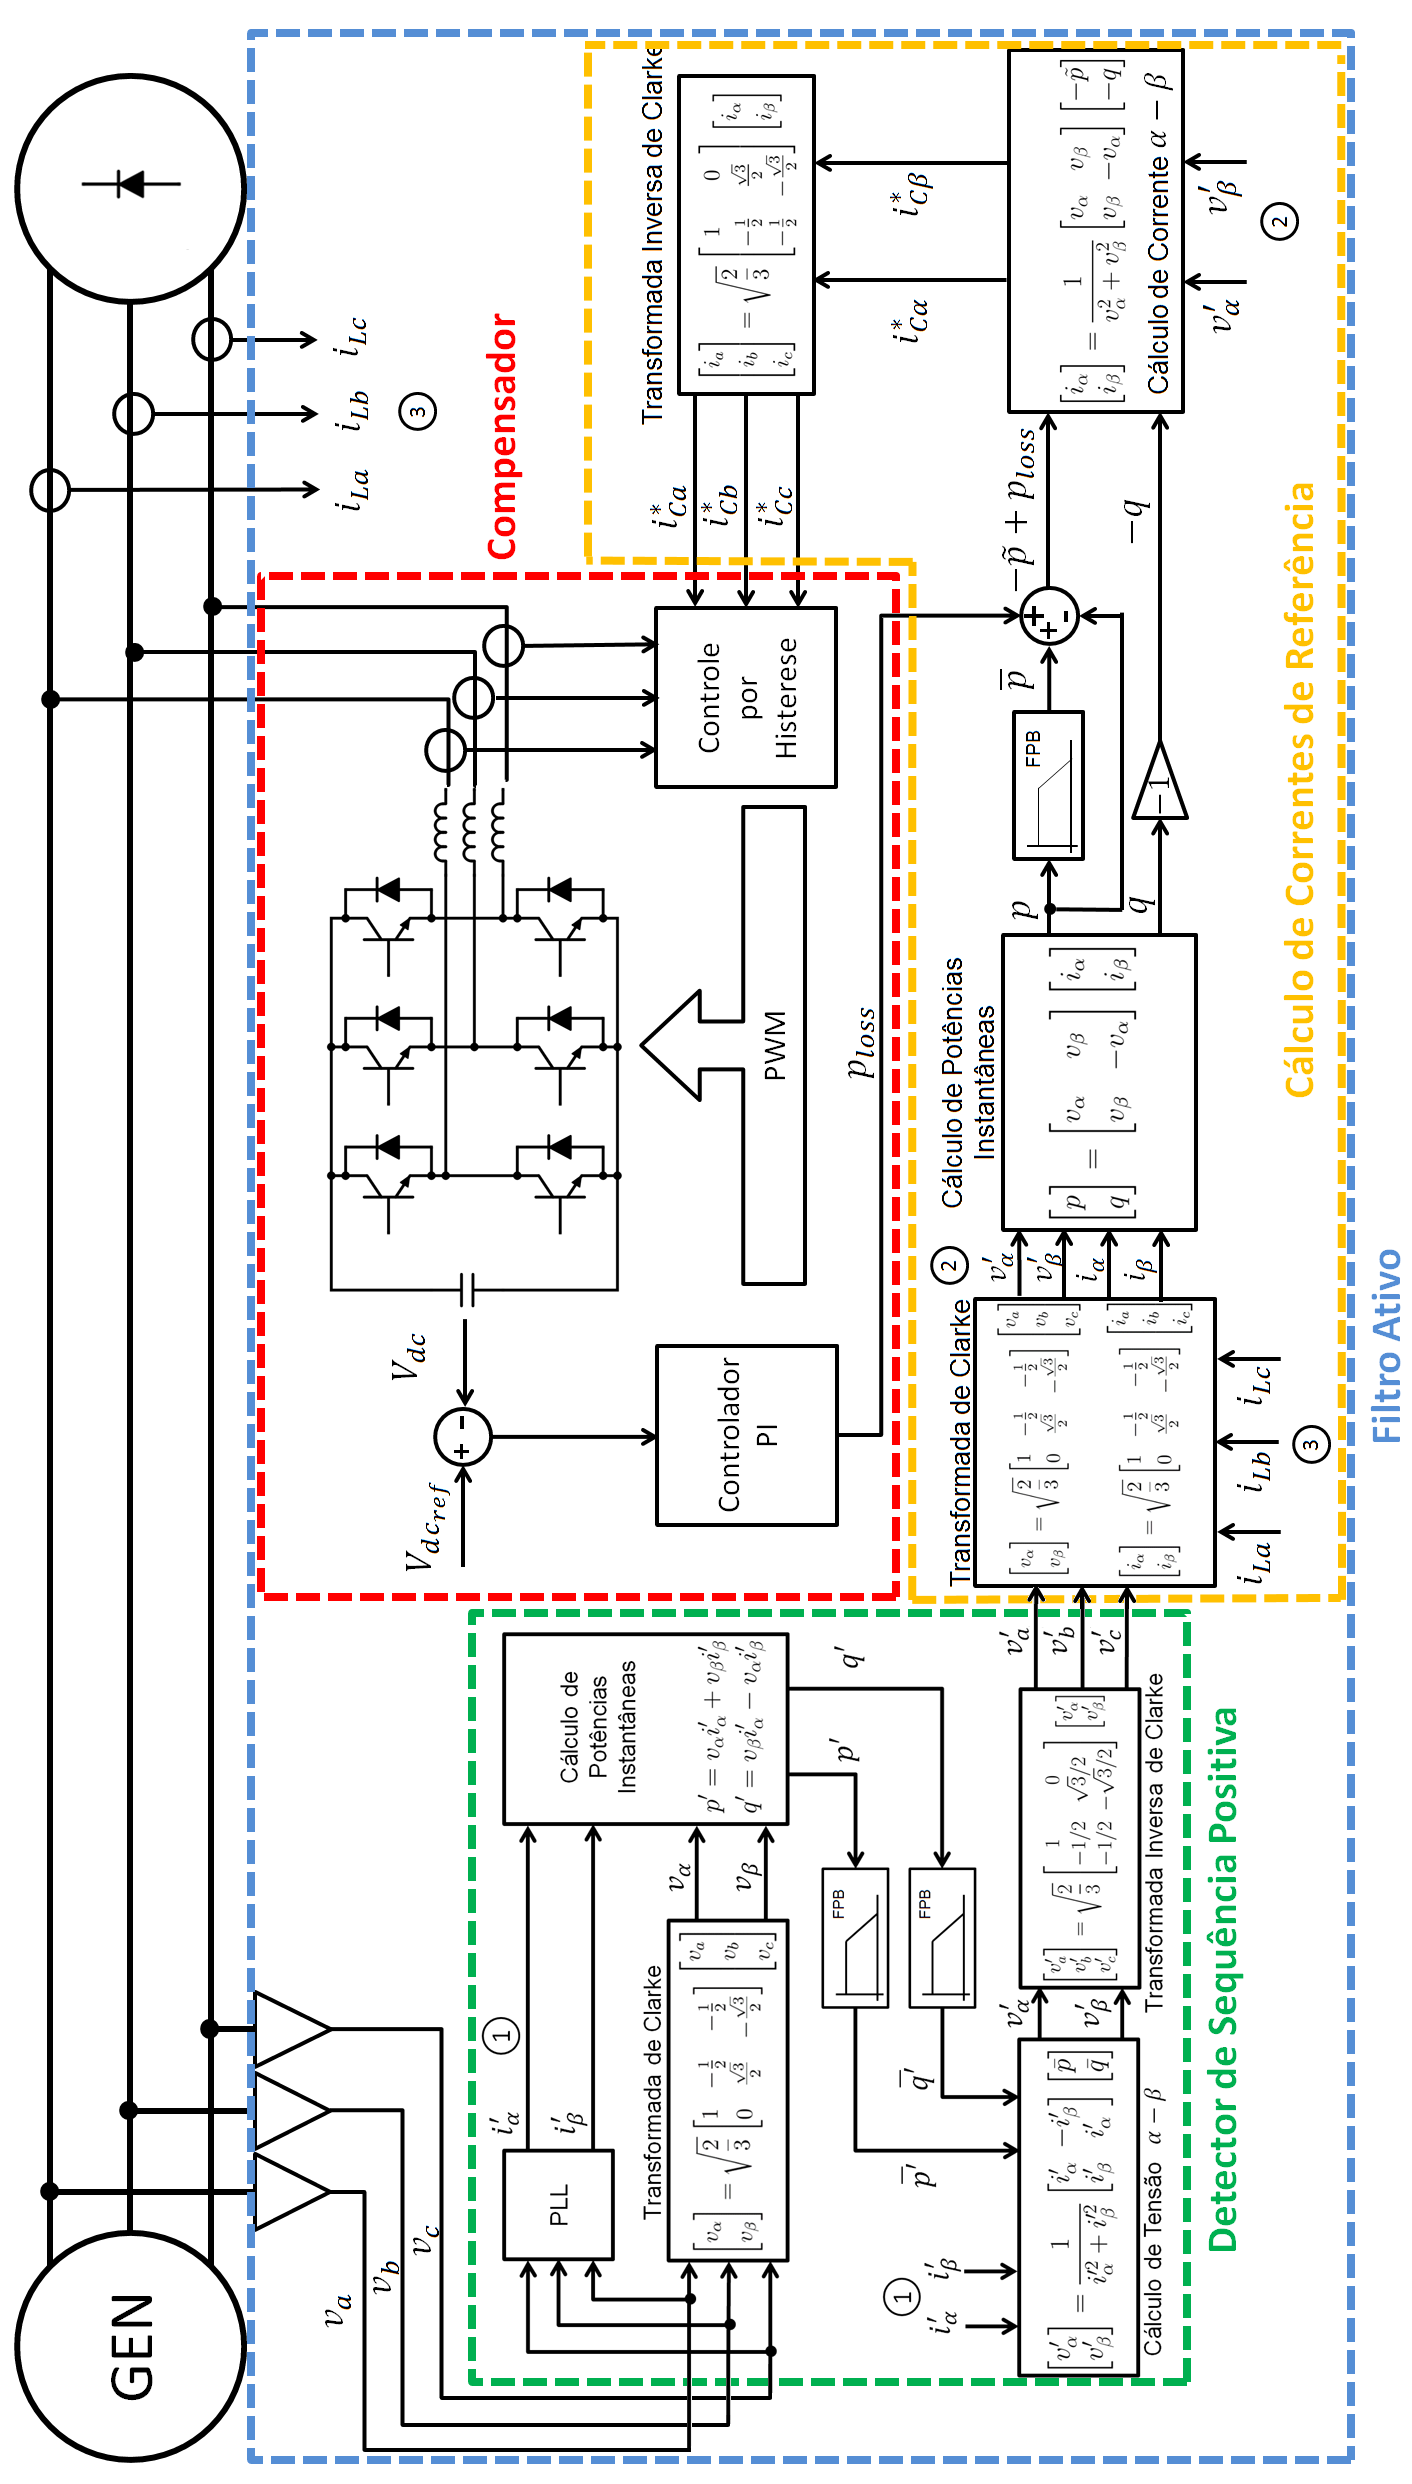
\includegraphics[height=0.98\textheight]{Cap4/Figuras/Tudao_lado_1.png}
	\caption{Sistema completo}
	\label{fig:Tudao_lado_1.png}
\end{figure}

Na Figura \ref{fig:Tudao_lado_1.png} pode ser observado o detector de sequ�ncia positiva, o bloco de c�lculo das correntes de refer�ncia atrav�s da utiliza��o da teoria das pot�ncias instant�neas, e o compensador. No compensador h� ainda a malha de controle de tens�o do capacitor do inversor, o comando do interruptores por controle por histerese e o inversor do tipo VSC, com sua respectiva indut�ncia de acoplamento e filtro capacitivo. Existe ainda os sensores de tens�o e corrente posicionados na rede para obten��o dos dados que s�o utilizados pelo filtro ativo e, por fim, existe ainda as indut�ncias na rede para compensar o fator de pot�ncia de deslocamento causado pelos filtros capacitivos presentes na sa�da do compensador.